\clearpage
%\begin{savequote}[8cm]
%\textlatin{Neque porro quisquam est qui dolorem ipsum quia dolor sit amet, consectetur, adipisci velit...}
%
%There is no one who loves pain itself, who seeks after it and wants to have it, simply because it is pain...
%  \qauthor{--- Cicero's \textit{de Finibus Bonorum et Malorum}}
%\end{savequote}

\chapter{\label{ch:6-interpretation}Extraction of CKM angle \Pgamma} 

\minitoc

The \CP observables from \btodkst decays are used to determine the physics parameters, \rb, \deltab and \Pgamma, via Eqs.~\ref{exp_Acp} - \ref{exp_Rpm4body}. In this determination, other parameters are taken from previous experiments to be used as external inputs. The coherence factor $\kappa$, discussed in Section \ref{sec:theory:gamma}, is estimated, as described in Section \ref{sec:interpretation:coherence}, and used as an extra constraint when determining \rb, \deltab and \Pgamma. The variations in acceptance across the four-body phase space and the effect of this on the interpretation is considered in Section \ref{sec:interpretation:inputs}. Section \ref{sec:interpretation:gammadini} discusses the determination of the physics parameters: \rb, \deltab and \Pgamma from measurements of \btodkst decays. Finally, Section \ref{sec:interpretation:futuresensitivity} discusses the expected sensitivity of the \btodkst channel to \rb, \deltab and \Pgamma, with an increased dataset after further running periods of the LHC.

\section{Coherence factor, $\kappa$}
\label{sec:interpretation:coherence}

Due to the large natural width of the \Kstarm meson, in the region near the \Kstarm mass interference may occur between the signal \Kstarm decay amplitude and amplitudes due to other \decay{\Bm}{\D\KS\pim} contributions, for example higher \KS\pim resonances and non-resonant decays. The presence of these interfering contributions when analysing the \btodkst decays dilutes the sensitivity to \Pgamma, which is quantified by a coherence factor, $\kappa$, where $0 \leq \kappa \leq 1$ and $\kappa = 1$ denotes a pure \Kstarm contribution, giving maximum sensitivity to \Pgamma. The parameter $\kappa$ is discussed in more detail in Section \ref{sec:theory:gamma}. 

In this section the parameter $\kappa$ is estimated in order to be used as an extra input, along with the \CP observables, in the extraction of \rb, \deltab and \Pgamma. The coherence factor $\kappa$ is estimated by developing an amplitude model for the \decay{\Bm}{\D\KS\pim} decay, and then using this model and the definition of $\kappa$, given in Equation \ref{kappadefinition}, to estimate $\kappa$ in this analysis.

\subsection{Decay model}
\label{sec:interpretation:model}

The role of the coherence factor, $\kappa$, in \btodkst decays is detailed in Section \ref{sec:theory:gamma}, where the definition of $\kappa$ is given by Equation \ref{kappadefinition}.

An amplitude model of \decay{\Bm}{\D X^-} decays is developed, where $X^-$ represents a resonant or non-resonant \KS\pim pair. In order to calculate $\kappa$, it is necessary to use the magntitudes and phases of the model components containing \decay{\bquark}{\uquark} transitions, $A_{\uquark\bquark}$, and \decay{\bquark}{\cquark} transitions, $A_{\cquark\bquark}$. The model contains resonant and non-resonant decays that are expected to contribute to in the region of phasespace used in this analysis, defined by the \Kstarm mass and \KS helicity angle requirements. The components of the model used for this study are:

\begin{itemize}
\item $\decay{\Bp}{\Dz K^*(892)^+}$ and $\decay{\Bp}{\Dzb K^*(892)^+}$
%\item $\decay{\Bp}{\Dz K^*(1410)^+}$ and $\decay{\Bp}{\Dzb K^*(1410)^+}$
\item $\decay{\Bp}{\Dz K^*_0(1430)^+}$ and $\decay{\Bp}{\Dzb K^*_0(1430)^+}$
\end{itemize}

A non resonant LASS component is used in the model, which is part of the $K^*_0(1430)^+$. Other resonances e.g. $K^*(1680)^+$ and $D_2^*(2460)^-$, are considered to be negligible in the region being considered and so are not included in the decay model. The parameters of the resonances are listed in Table \ref{resonances}.

\begin{table}[h]
\centering
\begin{tabular}{llll}
\hline
Resonance & Mass, M \mev & Width, $\Gamma$ \mev & Spin \\
\hline
$K^*(892)^+$ & $891.66 \pm 0.26$ & $50.8 \pm 0.9$ & 1 \\
%$K^*(1410)^+$ & $1414 \pm 15$ & $232 \pm 21$ & 1 \\
$K^*_0(1430)^+$ & $1425 \pm 50$ & $270 \pm 80$ & 0 \\
\hline
\end{tabular}
\caption{Parameters of the resonances in the decay model.}
\label{resonances}
\end{table}

The magnitudes $A_{\uquark\bquark}$ and $A_{\cquark\bquark}$ represent the amplitude of the suppressed and favoured \decay{\Bm}{\D X^-} decays, where $X^-$ represents a resonant or non-resonant \KS\pim pair. The amplitudes $A_{\uquark\bquark}$ and $A_{\cquark\bquark}$ are modelled as,
%The amplitude model was generated using the Laura++ package~\cite{Laura}.
\begin{align*}
A_{\uquark\bquark} =\ & a_{\uquark\bquark}^{K^*(892)^+}e^{-i\delta_{\uquark\bquark}^{K^*(892)^+}}RelBW(p;M_{K^*(892)^+},\Gamma_{K^*(892)^+},1)\ + \\
& a_{\uquark\bquark}^{K^*_0(1430)^+}e^{-i\delta_{\uquark\bquark}^{K^*_0(1430)^+}}LASS\_BW(p;M_{K^*_0(1430)^+},\Gamma_{K^*_0(1430)^+},0)\ + \\
& a_{\uquark\bquark}^{NR}e^{-i\delta_{\uquark\bquark}^{NR}}LASS\_NR
\end{align*}
and,
\begin{align*}
A_{\cquark\bquark} =\ & a_{\cquark\bquark}^{K^*(892)^+}e^{-i\delta_{\cquark\bquark}^{K^*(892)^+}}RelBW(p;M_{K^*(892)^+},\Gamma_{K^*(892)^+},1)\ + \\
& a_{\cquark\bquark}^{K^*_0(1430)^+}e^{-i\delta_{\cquark\bquark}^{K^*_0(1430)^+}}LASS\_BW(p;M_{K^*_0(1430)^+},\Gamma_{K^*_0(1430)^+},0)\ + \\
& a_{\cquark\bquark}^{NR}e^{-i\delta_{\cquark\bquark}^{NR}}LASS\_NR
\end{align*}
where, $RelBW$, $LASS\_BW$ and $LASS\_NR$ refer to the relativistic Breit-Wigner, LASS Breit-Wigner and LASS non-resonance shapes.% as implemented in Laura++~\cite{Laura}. 

The relative square of the magnitude of the various components is equal to the relative branching fractions in the limit of no interference. Therefore, it is assumed that the relative amplitudes are equal to the relative branching fractions. The only available branching fraction measurement is,
\begin{equation*}
\BF(\decay{\Bp}{\Dzb K^*(892)^+}) \times \BF(\decay{K^*(892)^+}{\KS\pip}) = 1.8 \times 10^{-4}
\end{equation*}

For the different resonant \Kstarp modes, it is assumed that they are produced with the same branching fraction as the $K^*(892)$ mode. The branching fractions of different resonant \Kstarp modes to the \KS\pip final state are also taken into account, namely $\BR(\decay{K^*(892)^+}{\KS\pip}) = \frac{1}{3}$ and $\BR(\decay{K^*_0(1430)^+}{\KS\pip}) = 0.31$.

The non-resonant branching fraction \BR(\decay{\Bp}{\Dzb\KS\pip}) is not known. Therefore, assuming,
\begin{equation*}
\frac{\BR(\decay{\Bz}{\Dm\Kz\pip})}{\BR(\decay{\Bz}{\Dm\Kzb\Kp})} = \frac{\BR(\decay{\Bp}{\Dzb\Kz\pip})}{\BR(\decay{\Bp}{\Dzb\Kzb\Kp})}
\end{equation*}
and using measurements for the other branching fractions~\cite{PDG2014}, the value of \BR(\decay{\Bp}{\Dzb\KS\pip}) is estimated to be $(5.2 \pm 0.3) \times 10^{-4}$.

When generating an amplitude model, only the relative amplitudes and phases of the various components are needed, therefore the $K^*(892)$ is fixed to have an amplitude of 1 and phase of 0. The relative amplitude $r_B$ is assumed to be 0.1. The values of the squares of the amplitudes $a_{\uquark\bquark}$ and $a_{\cquark\bquark}$ of the model components are taken in the ranges:

\begin{itemize}
\item \textbar $a_{\cquark\bquark}^{K^*(892)^+}$\textbar$^2 = 1$
%\item \textbar $a_{\cquark\bquark}^{K^*(1410)^+}$\textbar$^2 \in [0.7 \times 0.066,1.3 \times 0.066]$
\item \textbar $a_{\cquark\bquark}^{K^*_0(1430)^+}$\textbar$^2 \in [0.7 \times 0.93,1.3 \times 0.93]$
\item \textbar $a_{\cquark\bquark}^{NR}$\textbar$^2 \in [0.0,2.4]$
\end{itemize}

and,

\begin{itemize}
\item $a_{\uquark\bquark}^{K^*(892)^+} = r_B a_{\cquark\bquark}^{K^*(892)^+}$
%\item $a_{\uquark\bquark}^{K^*(1410)^+} = r_B a_{\cquark\bquark}^{K^*(1410)^+}$
\item $a_{\uquark\bquark}^{K^*_0(1430)^+} = r_B a_{\cquark\bquark}^{K^*_0(1430)^+}$
\item $a_{\uquark\bquark}^{NR} = r_B a_{\cquark\bquark}^{NR}$
\end{itemize}

Figure \ref{dalitzplot} shows an example of the amplitude model described. The \Kstar selection in this analysis, consisting of the \Kstar mass and \KS helicity angle requirements, are represented by dashed lines in this plot.

\begin{figure}[h]
\centering
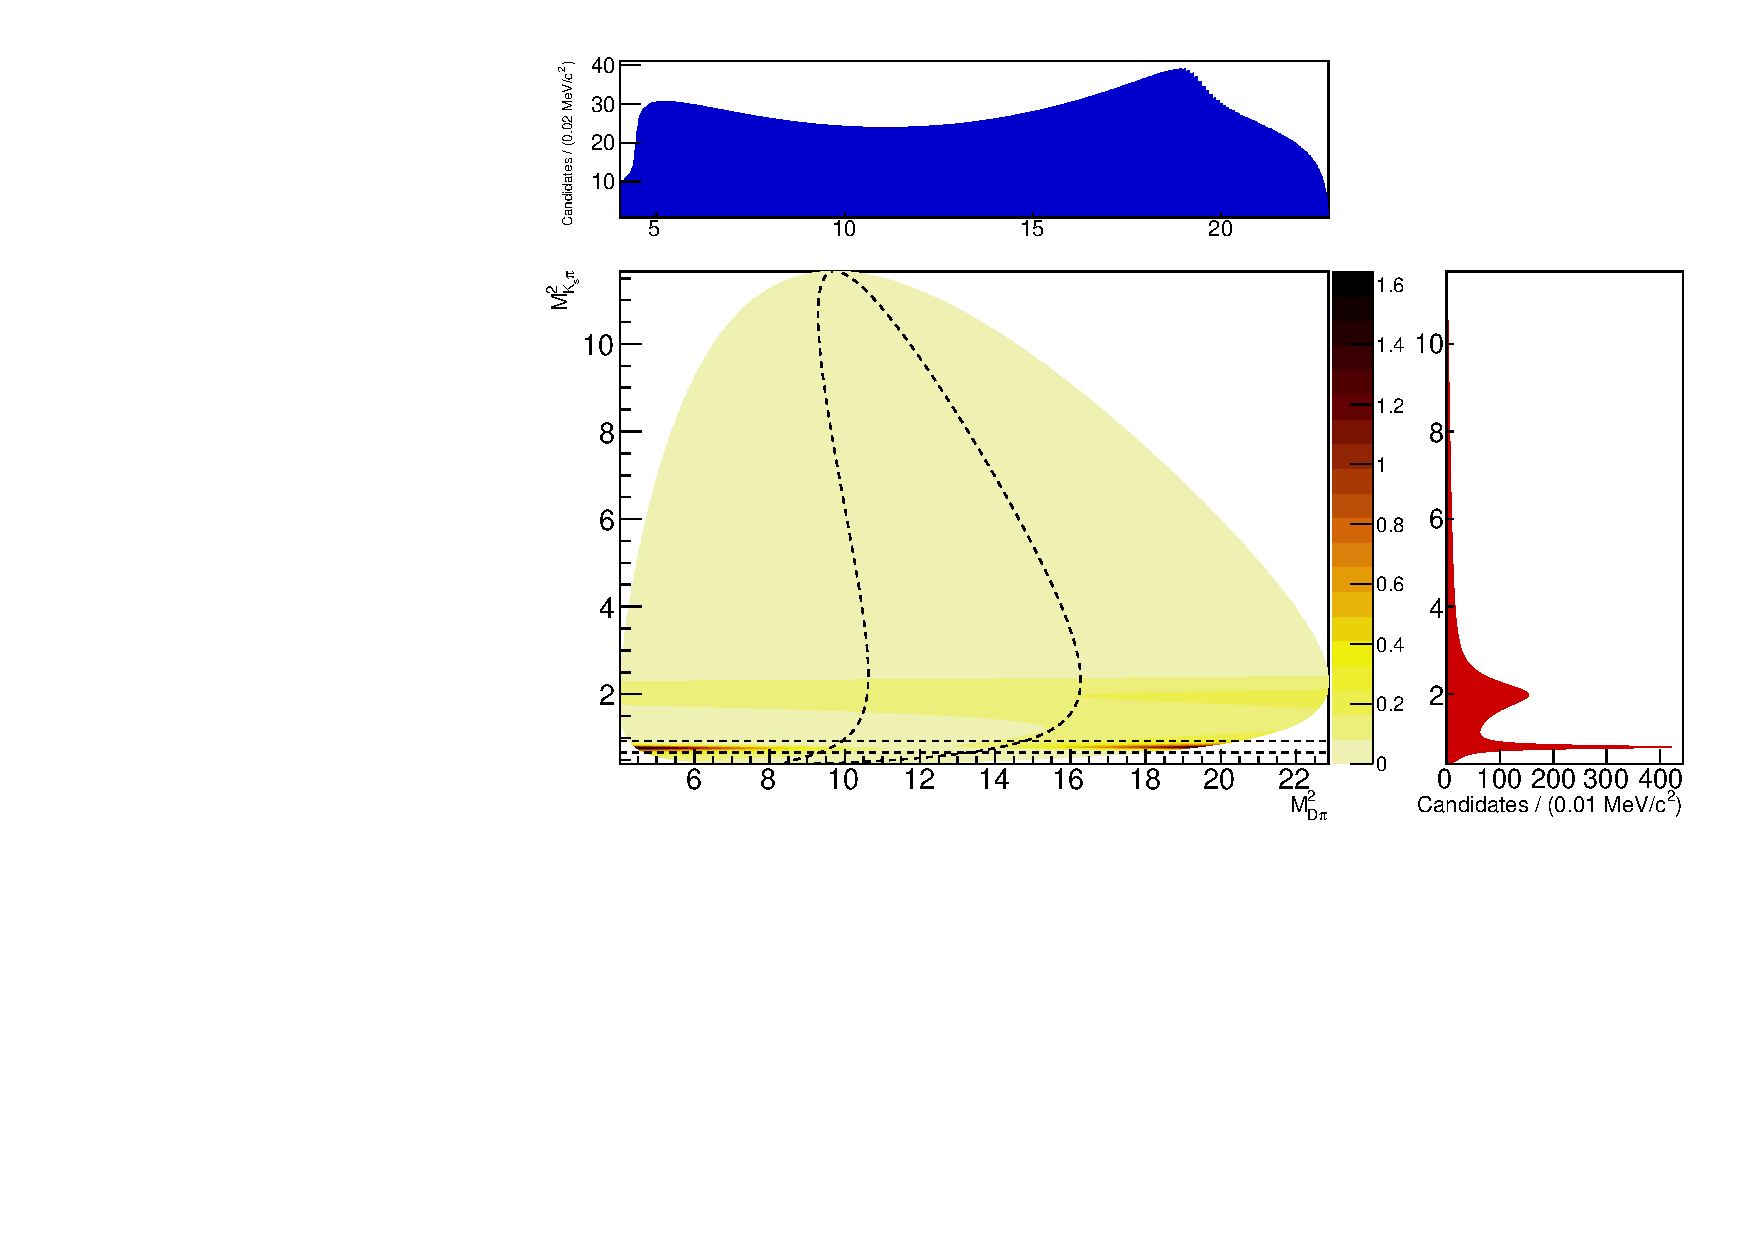
\includegraphics[width=0.8\linewidth]{figures/results/dalitz.pdf}
\caption{An example amplitude model used in the estimate of $\kappa$. The projections in the two Dalitz plot coordinates are shown. The dashed lines on the Dalitz plot represent the \Kstar mass and \KS helicity angle selection used in this analysis.}
\label{dalitzplot}
\end{figure}

\subsection{Estimation of the coherence factor, $\kappa$}
\label{sec:interpretation:kappa}

A large number of these amplitude models (1000) are generated, for each data sample the amplitudes and phases of the different resonances are varied within limits, as described by the decay model. The limits for the amplitudes are given in Section \ref{sec:interpretation:model} and all phases are generated randomly according to a flat distribution between $-\pi$ and $\pi$. The masses and widths of the resonances are kept constant at their central values, given in Table \ref{resonances}. 

For each Dalitz plot, $\kappa$ is computed as the magnitude of the expression in Equation \ref{kappadefinition}, resulting in a distribution of $\kappa$ values estimated by the model, as shown in Figure \ref{kappadistribution}. The mean and standard deviation of the resulting distribution is taken as an estimate of the central value and uncertainty of $\kappa$,  $0.95 \pm 0.04$. However, it is considered necessary to enhance the uncertainty of this estimate in order to account for the skewness of the distribution, therefore a final value of $0.95 \pm 0.06$ is used as an input in order to extract the physics parameters of interest.

\begin{figure}[h]
\centering
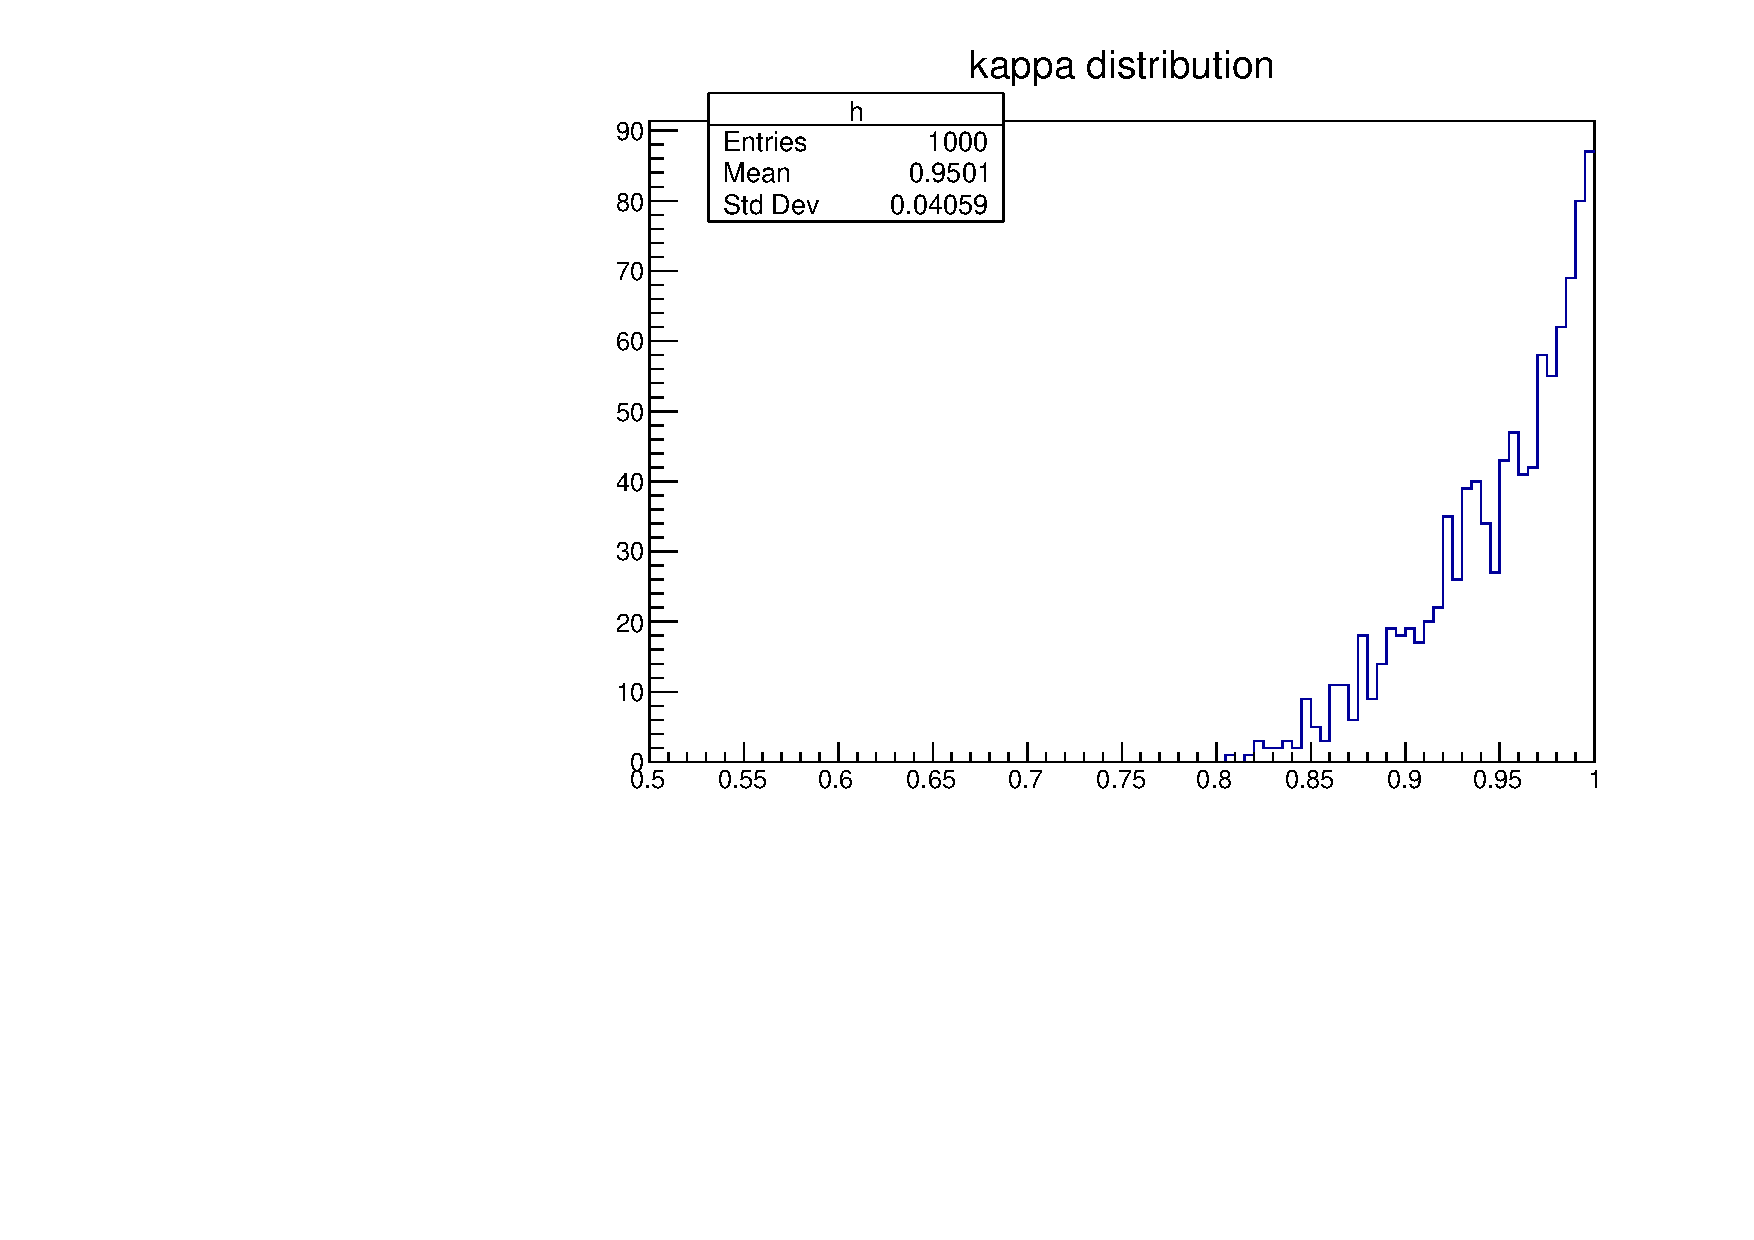
\includegraphics[width=0.5\linewidth]{figures/results/kappa.pdf}
\caption{Distribution of the measurements of $\kappa$ from 1000 pseudoexperiments.}
\label{kappadistribution}
\end{figure}

\section{Four-body phase space acceptance variations}
\label{sec:interpretation:inputs}

Several external inputs, relating to the \Dz decays, are required to interpret the results of the \CP observables from the \CP fit into information on $r_B$, $\delta_B$ and \Pgamma. The external parameters required are $r_D^{K\pi}$, $\delta_D^{K\pi}$, $r_D^{K3\pi}$, $\delta_D^{K3\pi}$, $R_{K3\pi}$ and $F_{4\pi}$. The parameters $R_{K3\pi}$ and $F_{4\pi}$ are to account for the fact that the four-body modes are not pure \CP or pure ADS modes. These parameters correspond to the fractional \CP content of the \decay{\Dz}{\pip\pim\pip\pim} decay, $F_{4\pi}$, and the coherence factor for the \decay{\Dz}{\Km\pip\pim\pip} decay, $R_{K3\pi}$. 

These parameters $F_{4\pi}$ and $R_{K3\pi}$ have been measured at CLEO and \lhcb measurements in Ref.~\cite{charmk3pi,LHCb-PAPER-2015-057,charm4pi}. However, the interpretation of \lhcb results have a dependence on \lhcb acceptance across the four-body phase space. Therefore the $F_{4\pi}$ and $R_{K3\pi}$ parameter values taken from CLEO may need to have corrections applied to be used for the interpretation of results from \lhcb. The difference in \lhcb acceptance across the four-body phase space would also affect the efficiency corrections for $A_{\pi\pi\pi\pi}$. These effects are expected to be negligible.

Figures \ref{dalitzk3pi} and \ref{dalitz4pi} show plots of projections of the four-body phase space distributions for \kpipipi and \pipipipi modes respectively. These plots are comparisons of distributions for simulated generator level signal distributions without any acceptance effects, and fully reconstructed simulated signal events used in this analysis. These distributions are very similar, which suggests that the use of the \kpipipi coherence factor, $R_{K3\pi}$, and fractional \CP content, $F_{4\pi}$, from CLEO can be used directly in the interpretation of \lhcb results. 

The value of $F_{4\pi}$, taken directly from the CLEO measurement, is $0.734 \pm 0.028$~\cite{charm4pi}. Based on similarities in acceptance compared to the \decay{\Bm}{\D\Km} analysis~\cite{B2DK_ADSGLW}, it is concluded that increasing the total uncertainty of $F_{4\pi}$ from 0.028 to 0.034 accounts for any uncertainty due to non-uniform \lhcb acceptance. Therefore, the value of $F_{4\pi}$ used as an input when determining $r_B$, $\delta_B$ and \Pgamma is $0.734 \pm 0.034$. Now considering the efficiency corrections to $A_{\pi\pi\pi\pi}$, a correction on the central value of $A_{\pi\pi\pi\pi}$ of ~1\% makes no significant difference to the results given that the statistical and systematic uncertainties are significantly larger than this correction. Therefore, it is concluded that small variations in efficiency lead to a negligible correction in the observables. 

\begin{figure}
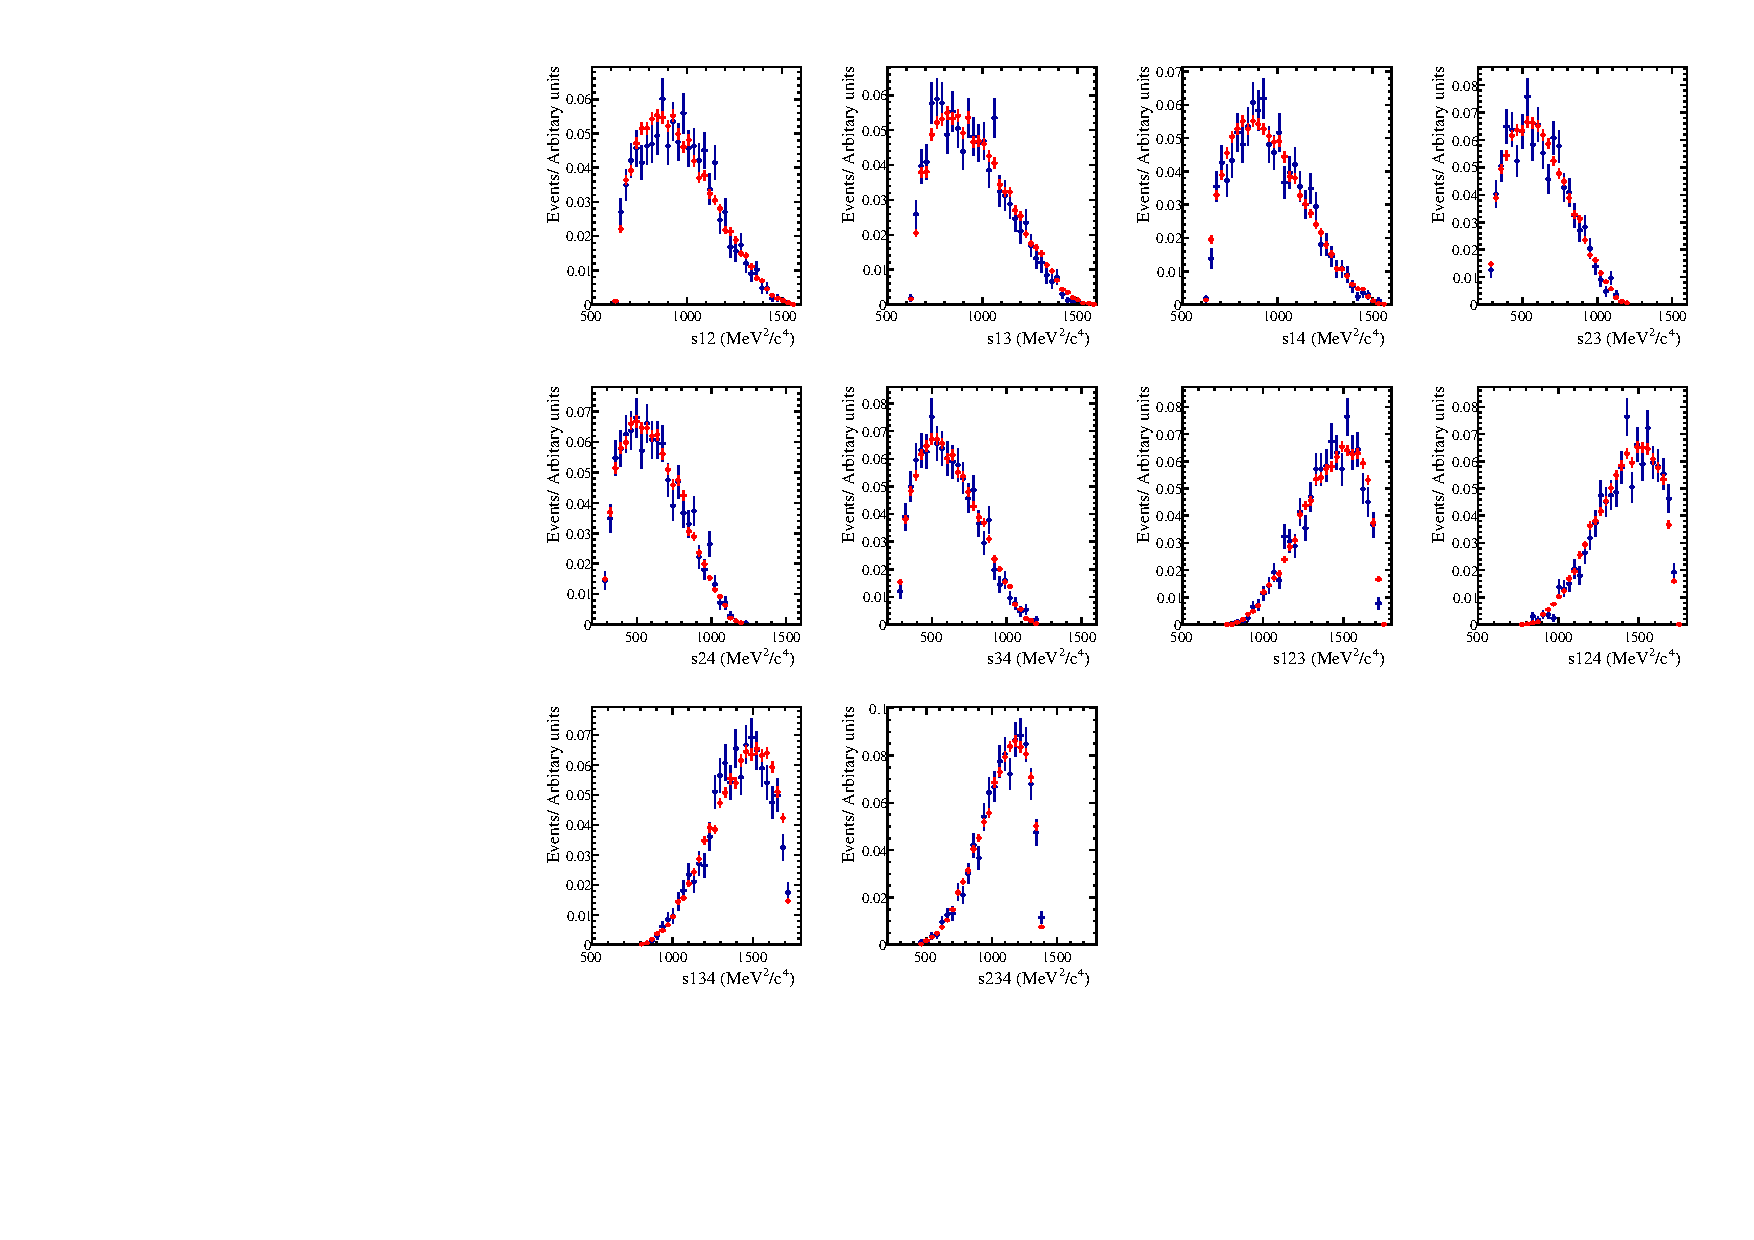
\includegraphics[width=\linewidth]{figures/results/dalitzDist_KPiPiPi.pdf}
\caption{Comparison of Dalitz variable distributions for simulation of generator level distributions (blue) and fully reconstructed selected events (red) in the \kpipipi mode.}
\label{dalitzk3pi}
\end{figure}

\begin{figure}
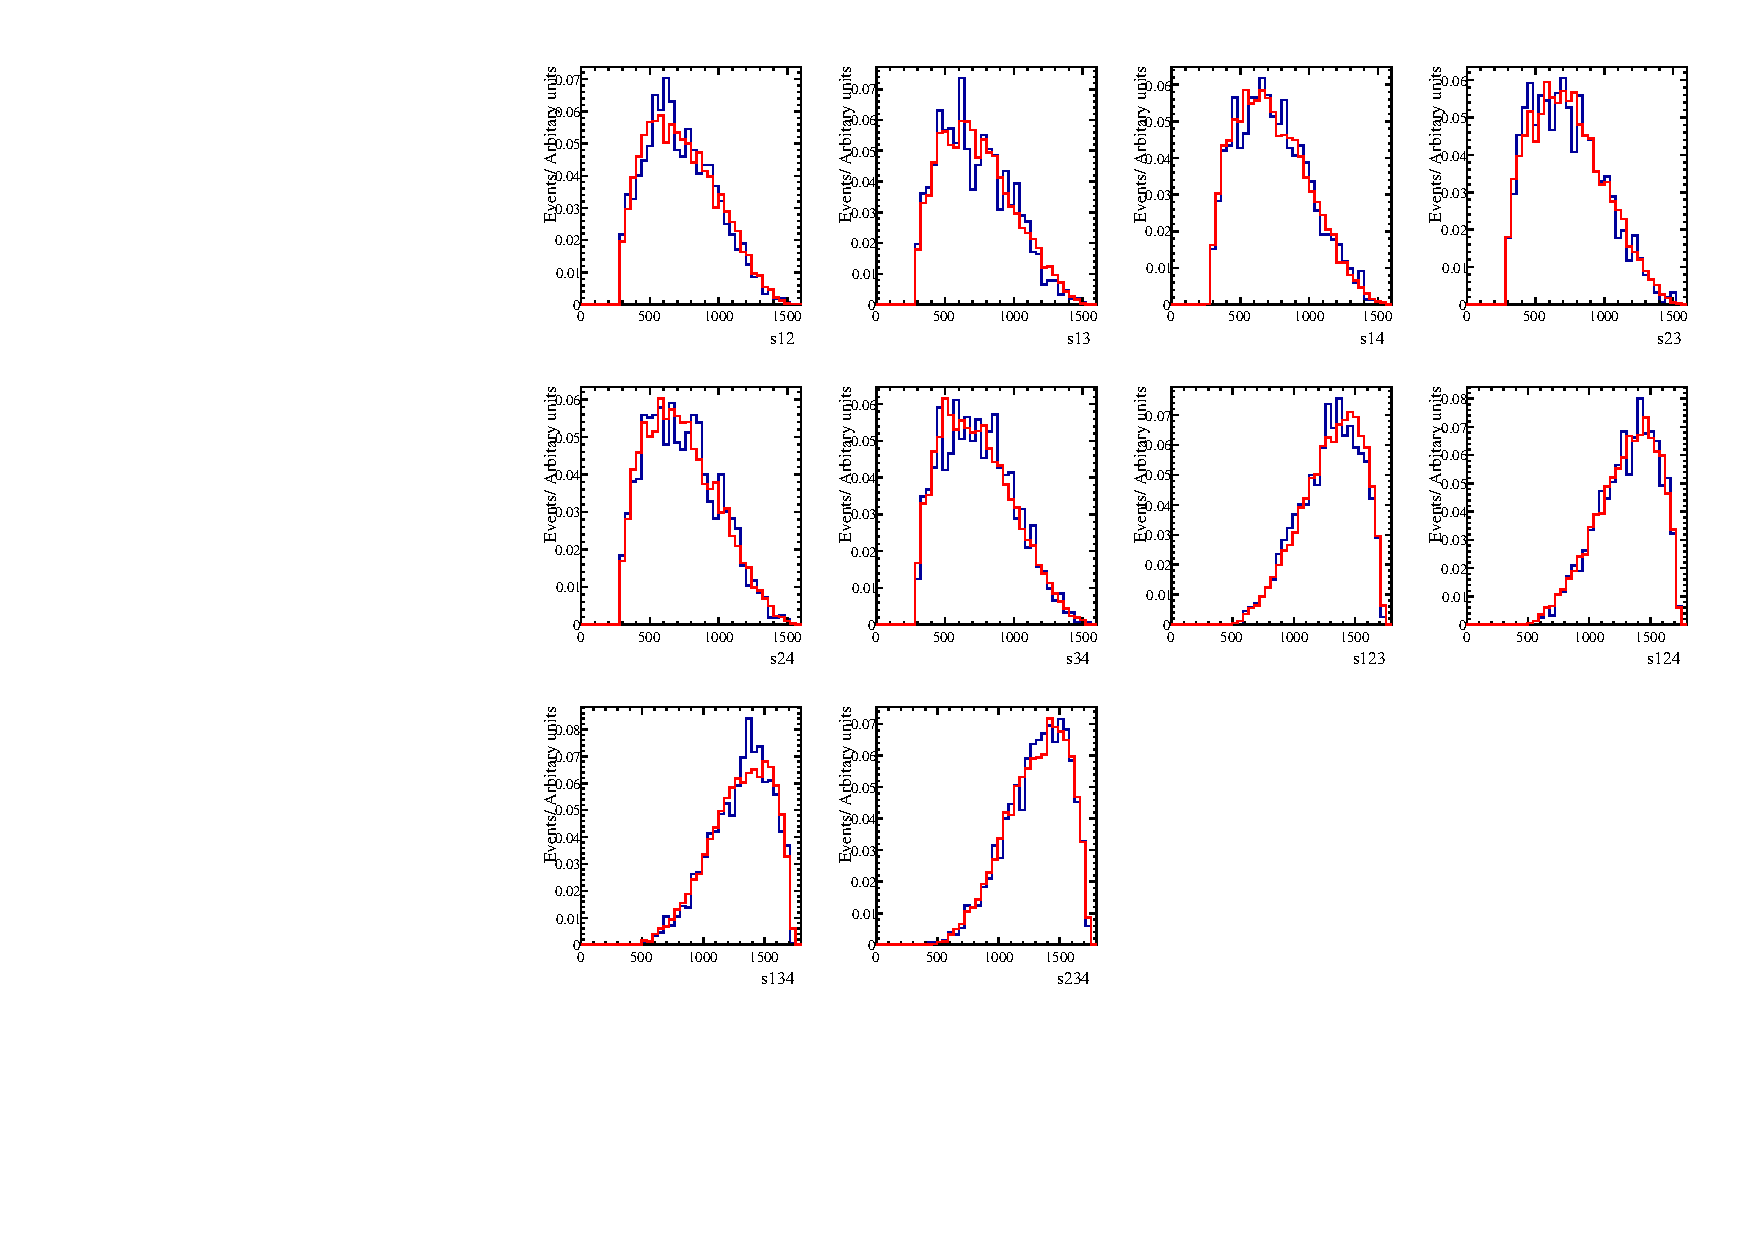
\includegraphics[width=\linewidth]{figures/results/dalitzDist_PiPiPiPi.pdf}
\caption{Comparison of Dalitz variable distributions for simulation of generator level distributions (blue) and fully reconstructed selected events (red) in the \pipipipi mode.}
\label{dalitz4pi}
\end{figure}

Further studies are performed to assess whether the parameters $R_{K3\pi}$ and $\delta_D^{K3\pi}$ require any corrections, when used in the interpretation, due to variations in acceptance over the four-body phase space. To assess the effects of small variation in the four-body phase space for \kpipipi decays, the coherence factor and strong phase are calculated from the \kpipipi amplitude models, both under the assumption of uniform acceptance and total \lhcb acceptance. The differences between these two scenarios give an estimate of the corrections that should be applied to the CLEO result before it is used in the \lhcb interpretation. The difference is calculated to be 0.002 for the coherence factor and 0.7$^{\circ}$ for the strong phase difference. The values of the inputs taken from CLEO/LHCb are $R_{K3\pi} = 0.43^{+0.17}_{-0.13}$ and $\delta_D^{K3\pi} = \left(128^{+28}_{-17}\right)$~\cite{charmk3pi}. Thereforer, the size of the shifts due to the \lhcb phase space acceptance are negligible in comparison to the CLEO uncertainties and hence no further action is taken.


\section{Results in terms of $r_B$, $\delta_B$ and \Pgamma}
\label{sec:interpretation:gammadini}

The \CP observables, measured in the \CP fit and listed in Section \ref{sec:cpfit:summary}, can be used to get a handle on the physics parameters of interest: $r_B$, $\delta_B$ and \Pgamma. These observables can be related to the physics parameters via Equations ~\ref{exp_Acp} - ~\ref{exp_Rpm4body}. The coherence factor is estimated, as described in the Section \ref{sec:interpretation:coherence}, and used as an input in the extraction of information on $r_B$, $\delta_B$ and \Pgamma. The parameters $r_D^{K\pi}$, $\delta_D^{K\pi}$, $r_D^{K3\pi}$, $\delta_D^{K3\pi}$, $R_{K3\pi}$ and $F_{4\pi}$ are required as external inputs and are taken from Ref.~\cite{HFAG,charmk3pi,LHCb-PAPER-2015-057,charm4pi}. The four-body \Dz decay mode \decay{\Dz}{\pip\pim\pip\pim} is an approximate \CP eigenstate, although as it is not a pure \CP eigenstate its sensitivity to \Pgamma is reduced. The parameter $F_{4\pi} \sim 0.75$~\cite{charm4pi} is the \CP-even fraction, which accounts for the dilution effect. Two-body \decay{\D}{\Kmp\pipm} decays are characterised by a single strong phase, however for multibody \decay{\D}{\Kmp\pipm\pimp\pipm} decays the strong phase varies over the phase space. By averaging the strong phase variation the interference effects are diluted, which is accounted for by the coherence factor, $R_{K3\pi}$. The \CP observables and other parameters are combined, and a minimisation is performed. The physics parameters involved are $r_B,\ \delta_B,\ \gamma,\ \kappa,\ r_D^{K\pi},\ \delta_D^{K\pi},\ r_D^{K3\pi},\ \delta_D^{K3\pi},\ F_{4\pi},\ R_{K3\pi}$ where $\kappa,\ r_D^{K\pi},\ \delta_D^{K\pi},\ r_D^{K3\pi},\ \delta_D^{K3\pi},\ F_{4\pi},\ R_{K3\pi}$ are constrained to their previously determined values. A global $\chi^2$ minimisation is performed where
\begin{equation}
\chi^2 = \sum_i \chi^2_i = (x(\theta) - x_0)^TV_0^{-1}(x(\theta)-x_0)
\end{equation}
In this expression, $x(\theta)$ is the set of observables calculated from the fundamental set of parameters $\theta$ and $x_0$ are the measured values. $V_0$ is the covariance matrix. The sensitivity of a given parameter is determined by calculating the $\chi^2$ at fixed points in parameter space. The difference between this $\chi^2$ value and that of the global minimum, quantifies the confidence in the global minimum. 

Using the measured values of the \CP observables, their uncertainties and the covariance matrices, a global $\chi^2$ minimisation is performed, resulting in a minimum $\chi^2$ of 3.0 with 9 degrees of freedom. A scan of physics parameters is performed for a range of values and the difference in $\chi^2$ between the parameter scan values and the global minimum, $\Delta\chi^2$, is evaluated. The confidence level for any pair of parameters is calculated assuming that these are normally distributed, which enables the $\Delta \chi^2 = 2.30,\ 6.18,\ 11.8$ contours to be drawn, corresponding to 68.3\%, 95.5\%, 99.7\% confidence levels, respectively. 

The results of the fit parameters is shown in Table \ref{gammadinifit}. Figures \ref{gammadiniplots2body} and \ref{gammadiniplotsallmodes} give the results as 2D contour plots of $r_B$ versus \Pgamma and $\delta_B$ versus \Pgamma. Figure \ref{gammadiniplots2body} shows the contour plots using the two-body modes only and Figure \ref{gammadiniplotsallmodes} show the contour plots using the observables from both the two- and four-body decays. The addition of the four-body modes slightly improves the constraints on the physics parameters, but in particular it provides additional distinction between the two minima. The data are consistent with the value of $\gamma$ indicated by previous measurements~\cite{LHCb-PAPER-2016-032, CKMFitter}, $\sim 70^\circ$. The values of $r_B$, $\delta_B$ and \Pgamma are determined at the point where the global $\chi^2$ of the fit is minimised. Calculating the values of $r_B$, $\delta_B$ and \Pgamma from running 100 pseudoexperiments gives values of:
\begin{align*}
r_B &= 0.113^{+0.015}_{-0.021} \\
\delta_B &= \left(43.3^{+19.0}_{-19.0}\right)^{\circ} \\
\Pgamma &= \left(40.0^{+18.0}_{-16.0}\right)^{\circ} 
\end{align*}

These confidence level distributions for $r_B$, $\delta_B$ and \Pgamma are not Gaussian beyond 1$\sigma$, and $\delta_B$ and \Pgamma contain a second minimum, as can be seen from Figure \ref{gammadiniplotsallmodes}, therefore the results quoted cannot be extrapolated to consider 2$\sigma$ or 3$\sigma$ values. 

\begin{figure}[h]
\centering
\subfloat[$r_B$ versus \Pgamma]{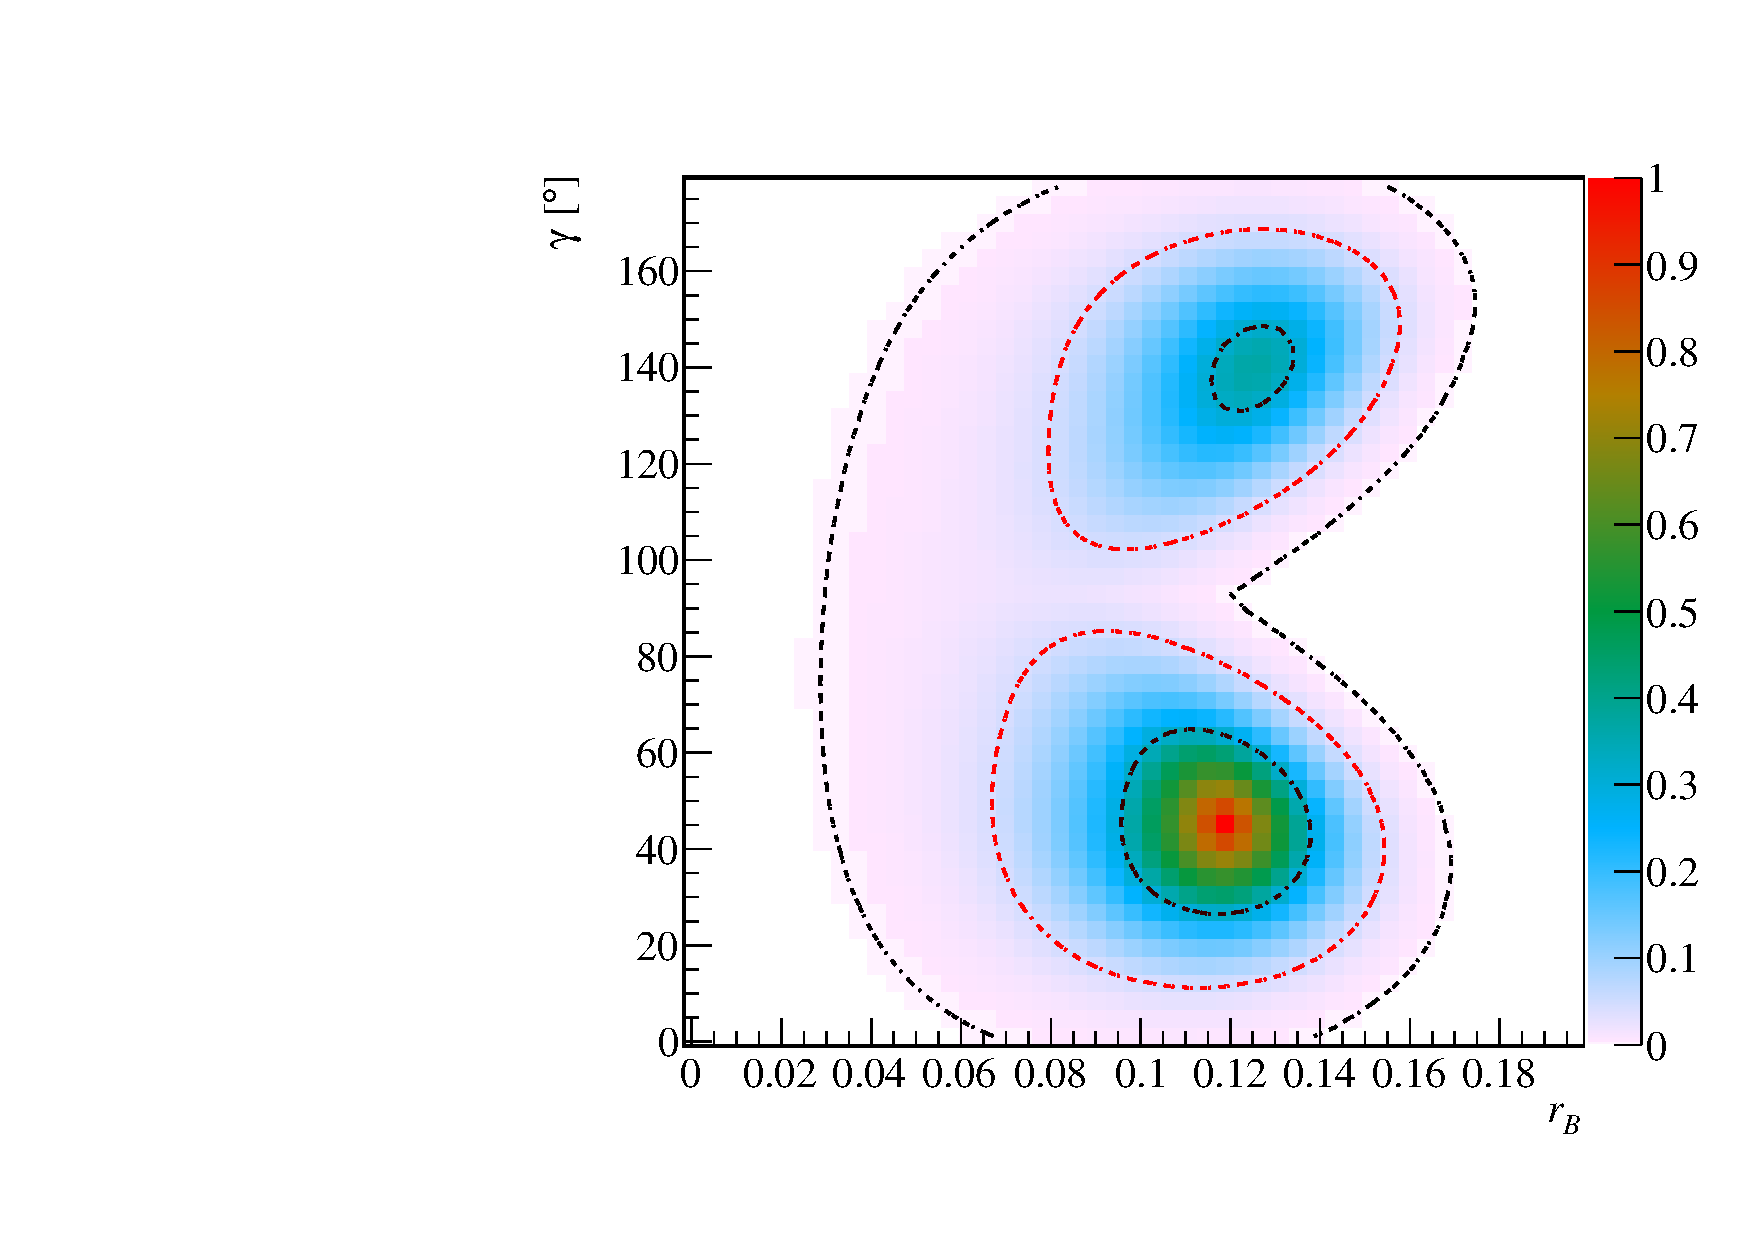
\includegraphics[width=0.5\linewidth]{figures/interpretation/rBu_dkstar_gamma_2Dscan_nomixing_2body.pdf}}
\subfloat[$\delta_B$ versus \Pgamma]{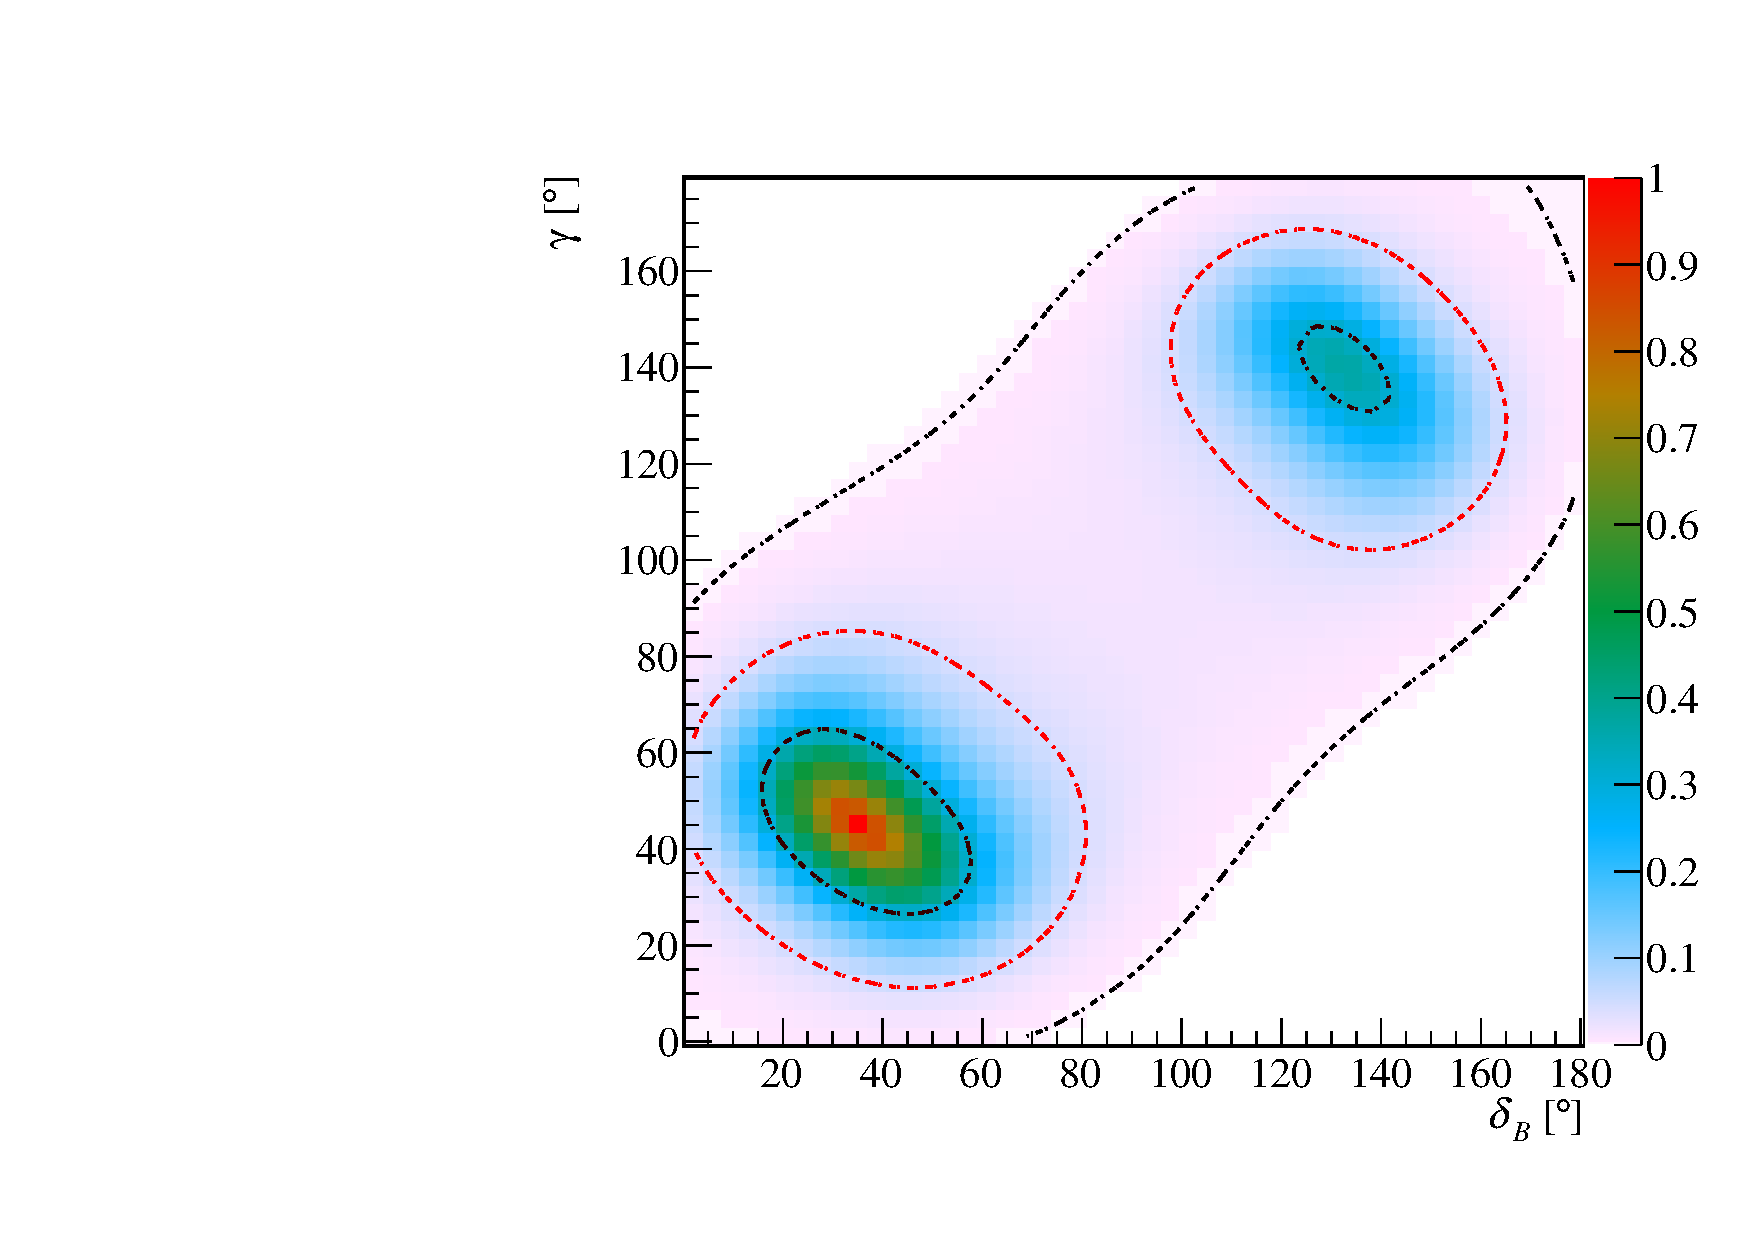
\includegraphics[width=0.5\linewidth]{figures/interpretation/deltaBu_dkstar_gamma_2Dscan_nomixing_2body.pdf}}
\caption{2D contour plots using the two-body modes only}
\label{gammadiniplots2body}
\end{figure}

\begin{figure}[h]
\centering
\subfloat[$r_B$ versus \Pgamma]{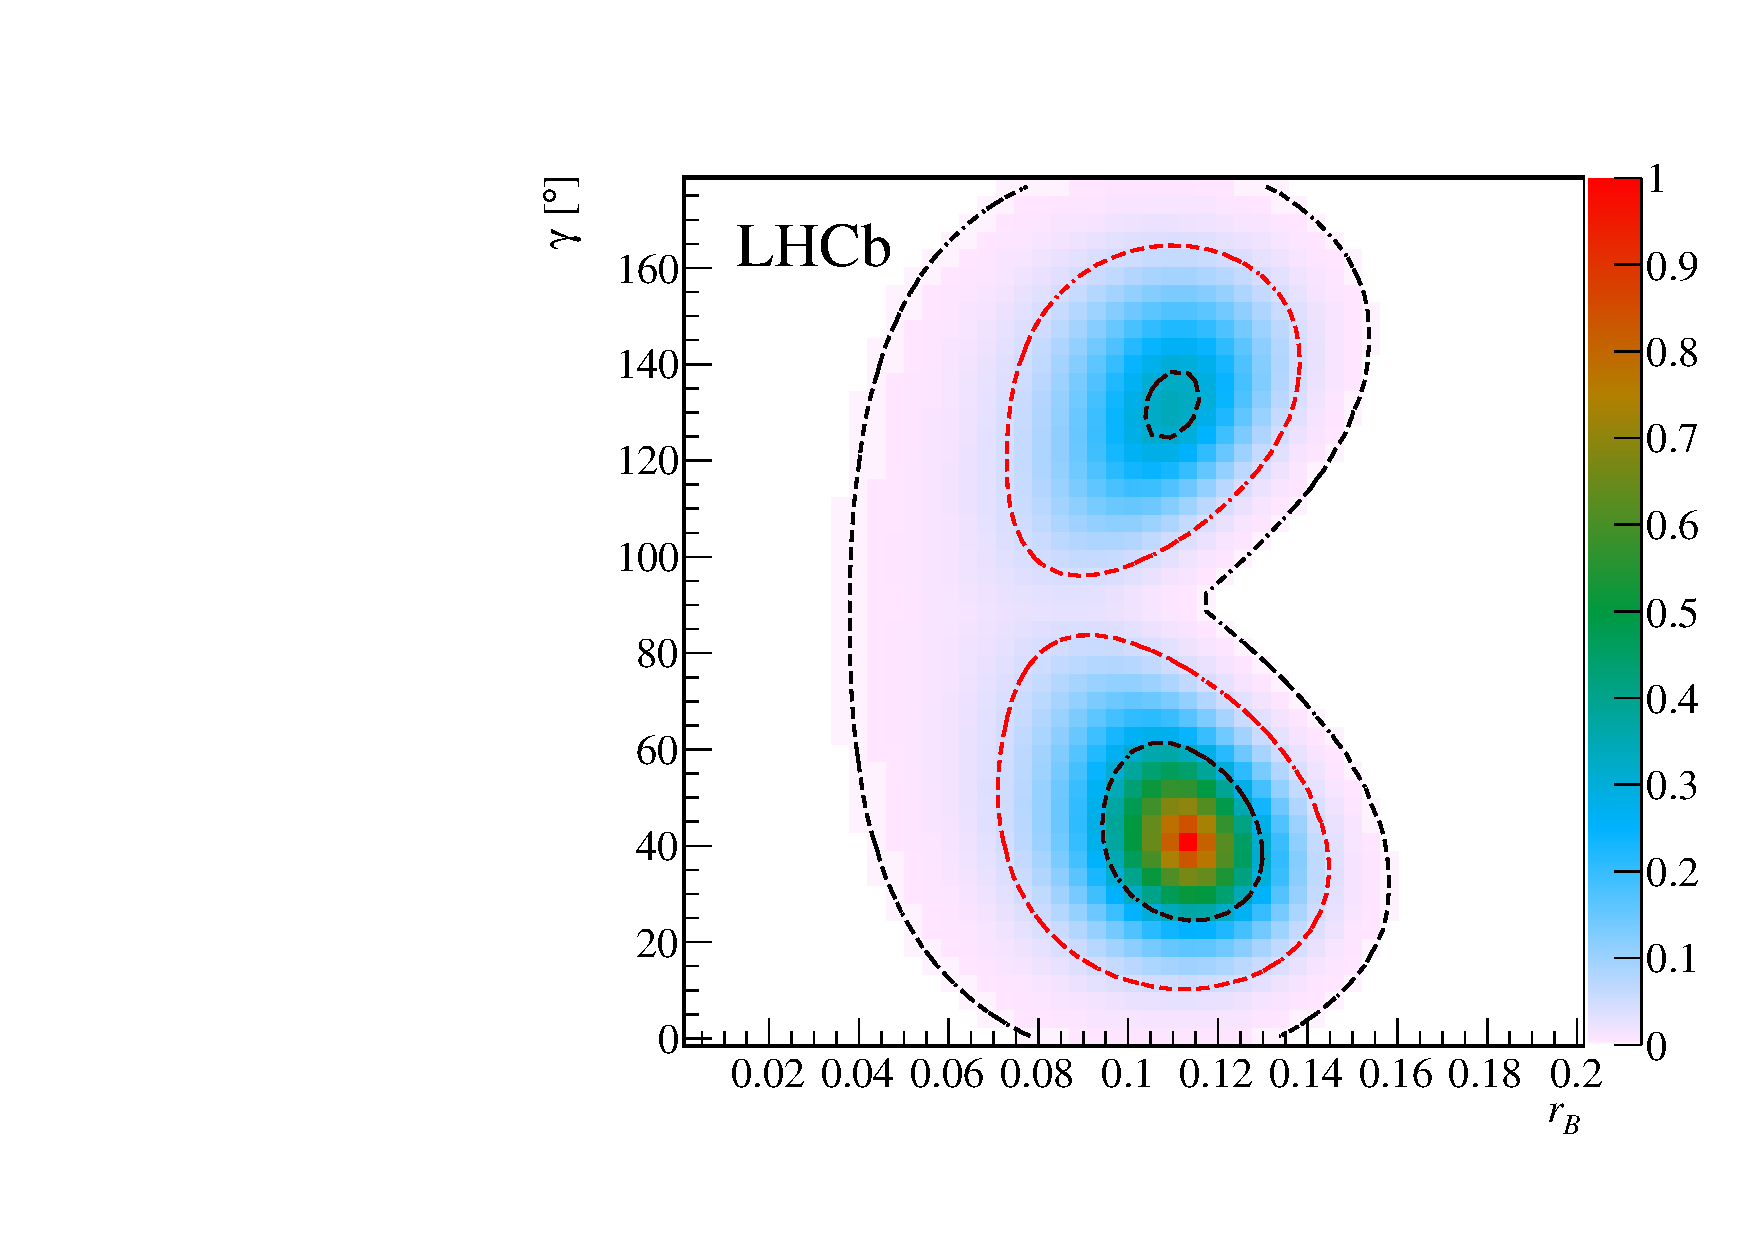
\includegraphics[width=0.5\linewidth]{figures/interpretation/rBu_dkstar_gamma_2Dscan_nomixing_all.pdf}}
\subfloat[$\delta_B$ versus \Pgamma]{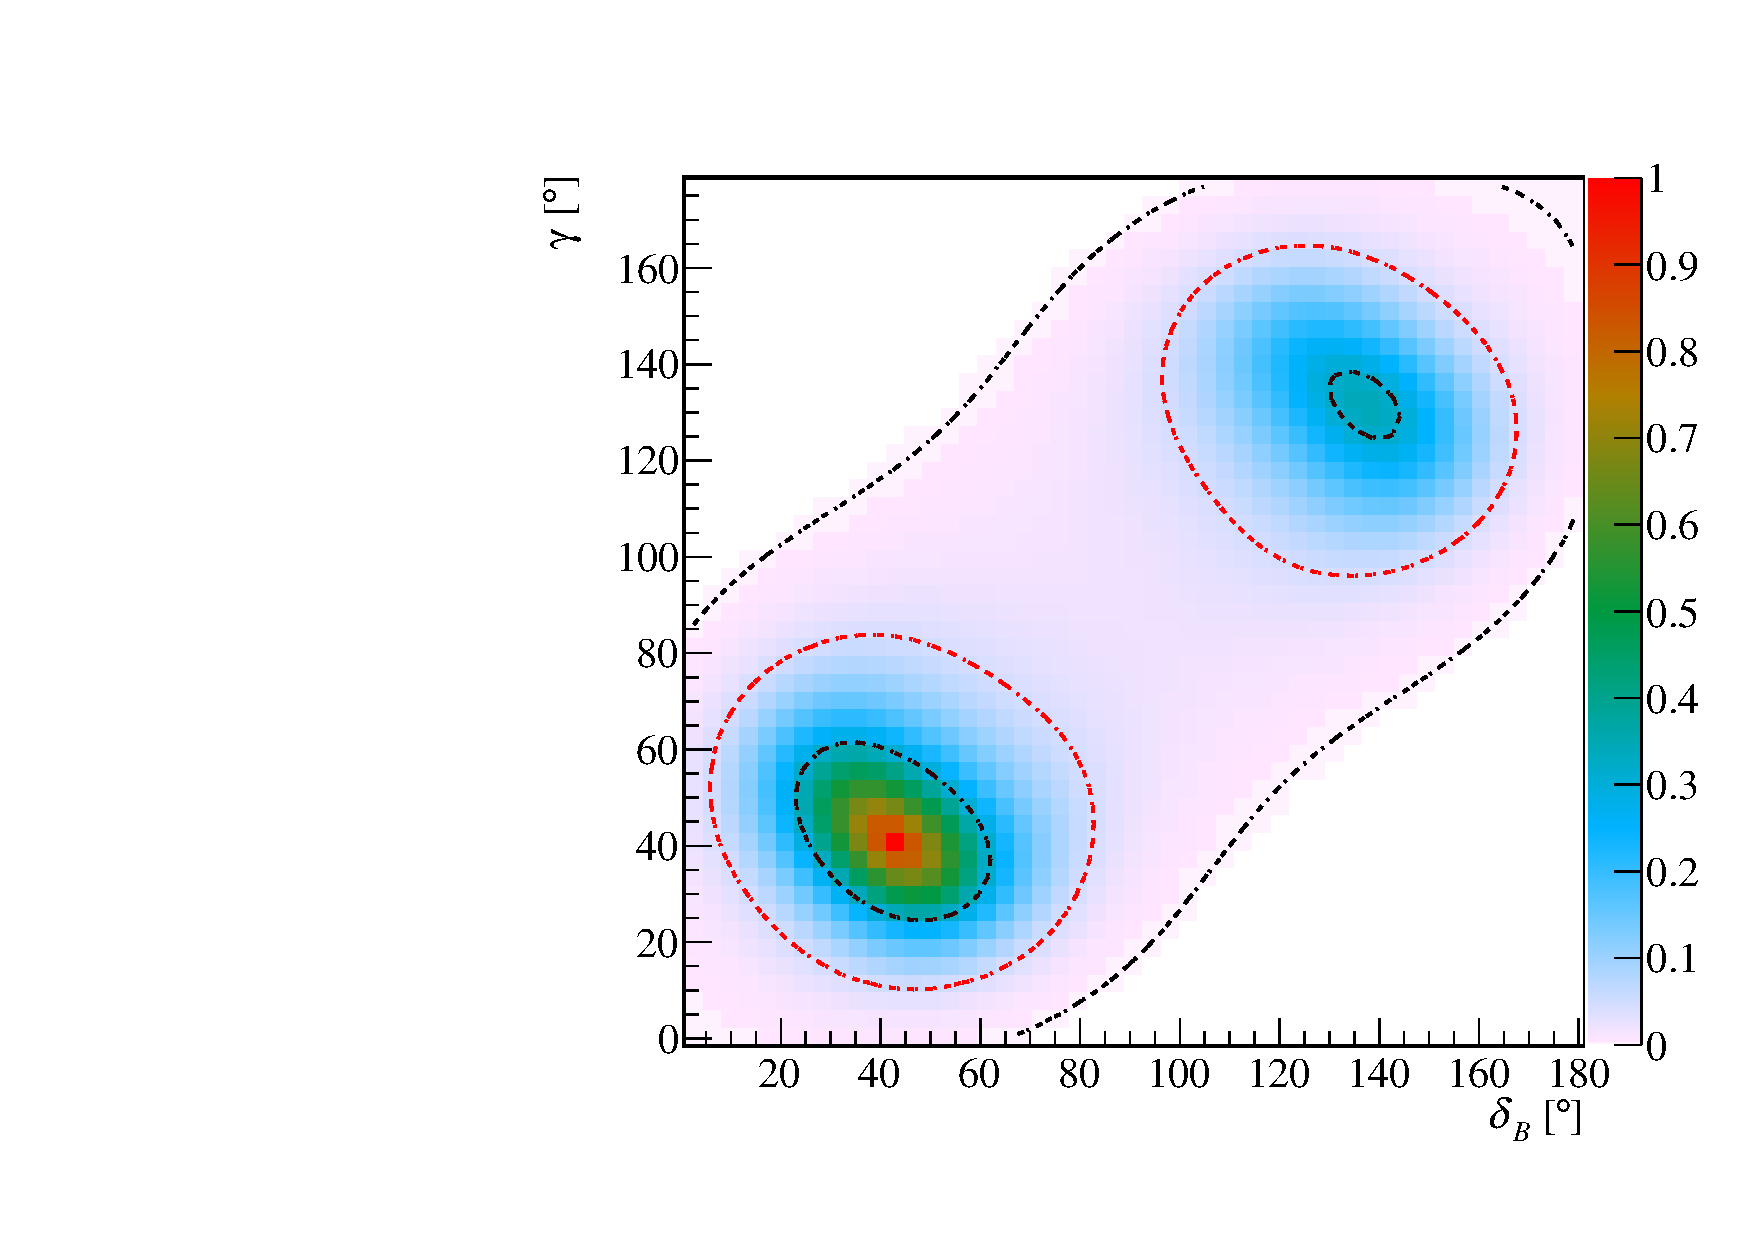
\includegraphics[width=0.5\linewidth]{figures/interpretation/deltaBu_dkstar_gamma_2Dscan_nomixing_all.pdf}}
\caption{2D contour plots using both the two- and four-body modes}
\label{gammadiniplotsallmodes}
\end{figure}

\begin{table}
\centering
\begin{tabular}{cccc}
Fit parameter & Value & Negative error & Positive error \\
\hline
\Pgamma & 41 & -16 & 19 \\
$r_B$ & 0.113 & -0.019 & 0.016 \\
$\delta_B$ & 43 & -20 & 19 \\
$\kappa$ & 0.96 & -0.06 & 0.06 \\
$r_D^{K\pi}$ & 0.0591 & -0.0003 & 0.0003 \\
$\delta_D^{K\pi}$ & 193 & -11 & 11 \\
$r_D^{K3\pi}$ & 0.0549 & -0.0006 & 0.0006 \\
$\delta_D^{K3\pi}$ & 134 & -22 & 22 \\
$R_{K3\pi}$ & 0.44 & -0.15 & 0.15 \\
$F_{CP}$ & 0.74 & -0.03 & 0.03
\end{tabular}
\caption{Results of fit parameters}
\label{gammadinifit}
\end{table}

\section{Expected future sensitivity to $r_B$, $\delta_B$ and \Pgamma}
\label{sec:interpretation:futuresensitivity}

The \btodkst mode has shown an increase of three times the yield per unit integrated luminosity from \runone to \runtwo, mainly due to the increase in centre of mass energy of the $pp$ collisions from 7 and 8\tev to 13\tev. As previously stated, the data used in this analysis was collected in 2011 and 2012, forming the \runone \dataset, and 2015 and 2016, forming the \runtwo \dataset. The current running period of the LHC, namely \runtwo, is currently ongoing. The projected yields for the end of Run 2 and the end of Run 3 can be estimated using the forecasts for the stored integrated luminosity during these data taking periods. These projections can be found in \tab~\ref{projectedyields}. In order to do this assumptions that the yield per unit integrated luminosity remains the same for the rest of \runtwo and for Run 3. The projections for Run 3 have large errors as the centre of mass energy may increase to 14\tev, resulting in an increase in the yield per unit integrated luminosity, and the collected integrated luminosity is very speculative. Also, between Run 2 and Run 3 many upgrades to the detector will be performed, which have not been taken into account for these projections.

\begin{table}
\resizebox{\textwidth}{!}{
\begin{tabular}{cccc}
Year & Integrated Luminosity & \kpi yield & Yield per \invfb \\
\hline
\runone & 3\invfb & 725 & 242 \\
\runtwo (up to 2016) & 1.8\invfb & 1390 & 771 \\
\runtwo (after 2016) & 1.6\invfb & 1233 & 771 \\
Run 3 & 14\invfb & 10800 & 771 \\
\end{tabular}}
\caption{Projected yields}
\label{projectedyields}
\end{table}

Using the assumptions made in \tab~\ref{projectedyields}, the projected future sensitivity to the physics parameters \rb, \deltab and \Pgamma can be estimated. Figure \ref{gammadiniplotsrun2} gives the projected results at the end of Run 2 as 2D contour plots of \rb versus \Pgamma and \deltab versus \Pgamma. The equivalent plots are shown in Figure \ref{gammadiniplotsrun3} for the end of Run 3. 

\begin{figure}[h]
\centering
\subfloat[\rb versus \Pgamma]{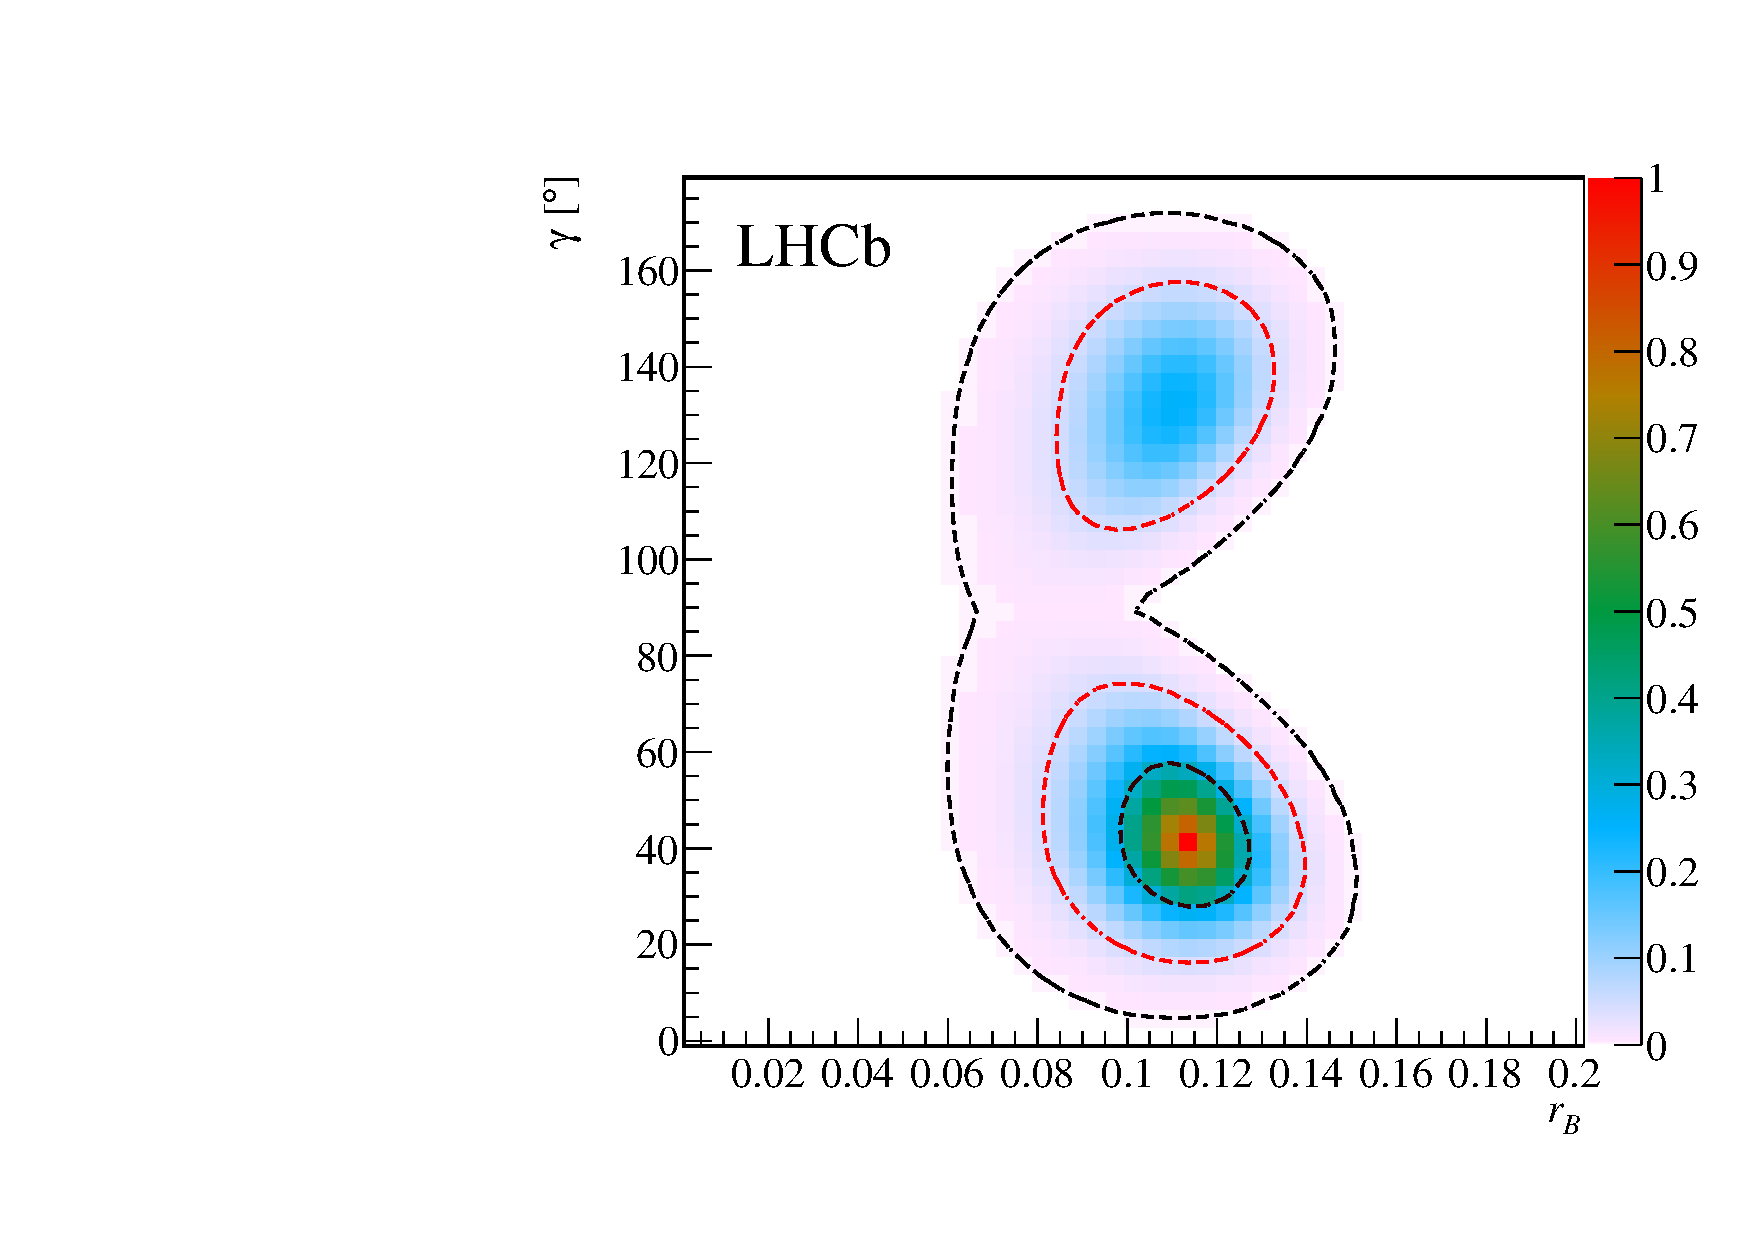
\includegraphics[width=0.5\linewidth]{figures/interpretation/rBu_dkstar_gamma_2Dscan_nomixing_endofrun2.pdf}}
\subfloat[\deltab versus \Pgamma]{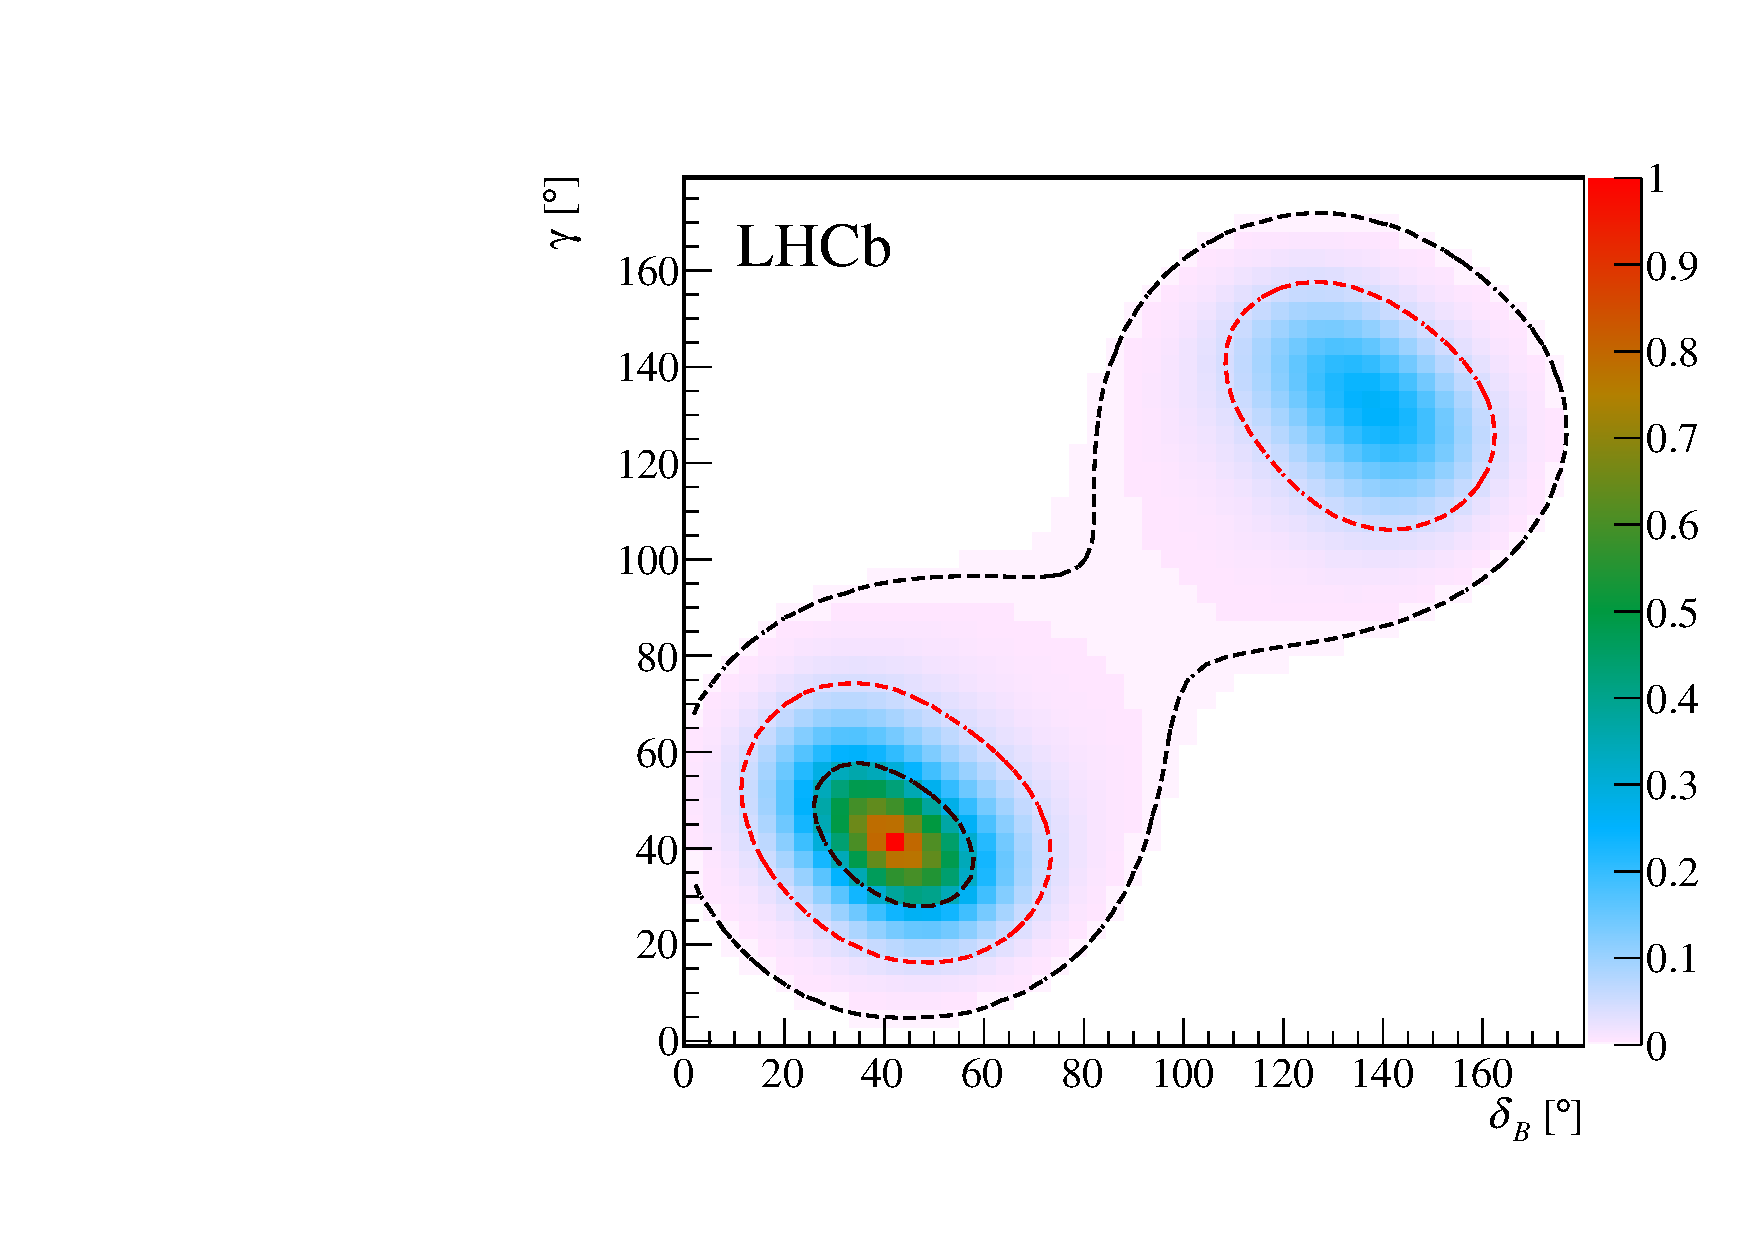
\includegraphics[width=0.5\linewidth]{figures/interpretation/deltaBu_dkstar_gamma_2Dscan_nomixing_endofrun2.pdf}}
\caption{2D contour plots projected to the end of \runtwo assuming the central values remain the same.}
\label{gammadiniplotsrun2}
\end{figure}

\begin{figure}[h]
\centering
\subfloat[\rb versus \Pgamma]{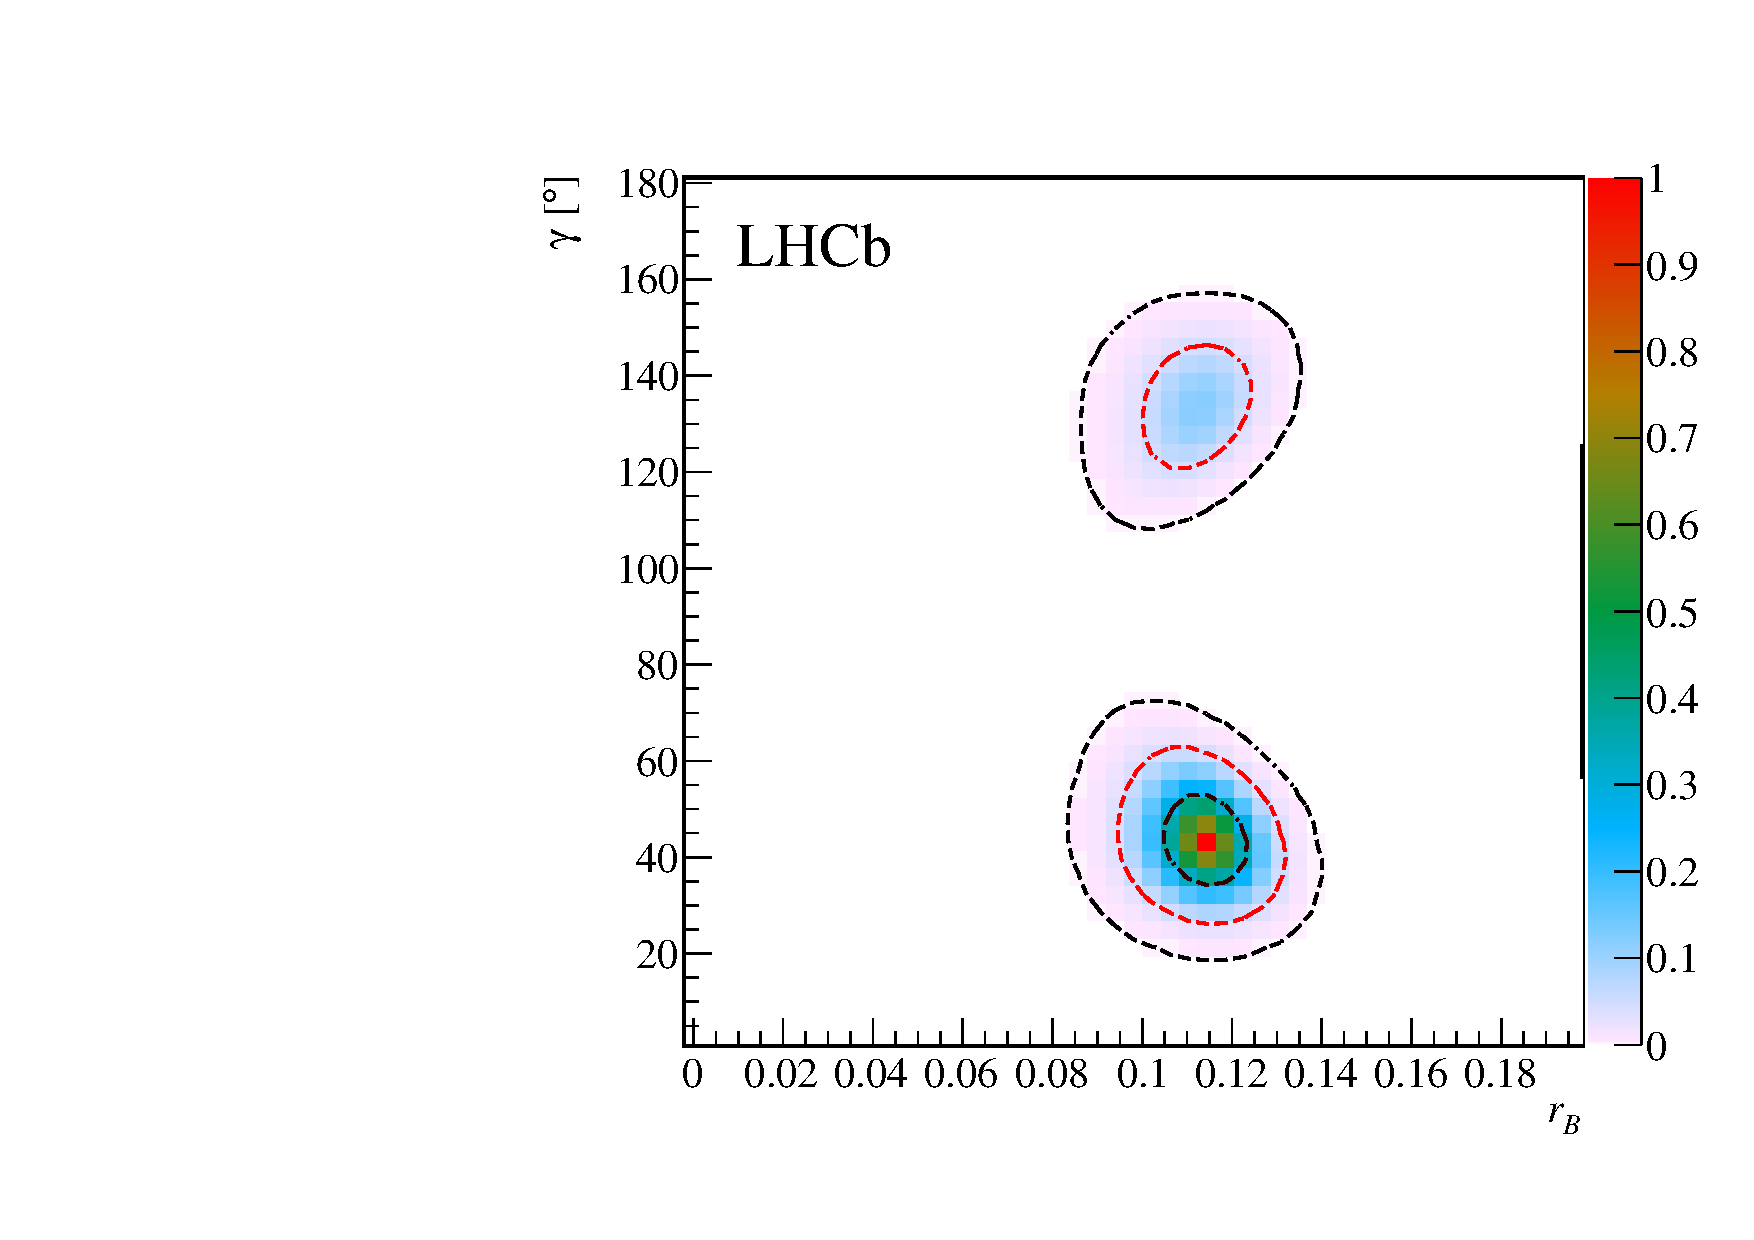
\includegraphics[width=0.5\linewidth]{figures/interpretation/rBu_dkstar_gamma_2Dscan_nomixing_endofrun3.pdf}}
\subfloat[\deltab versus \Pgamma]{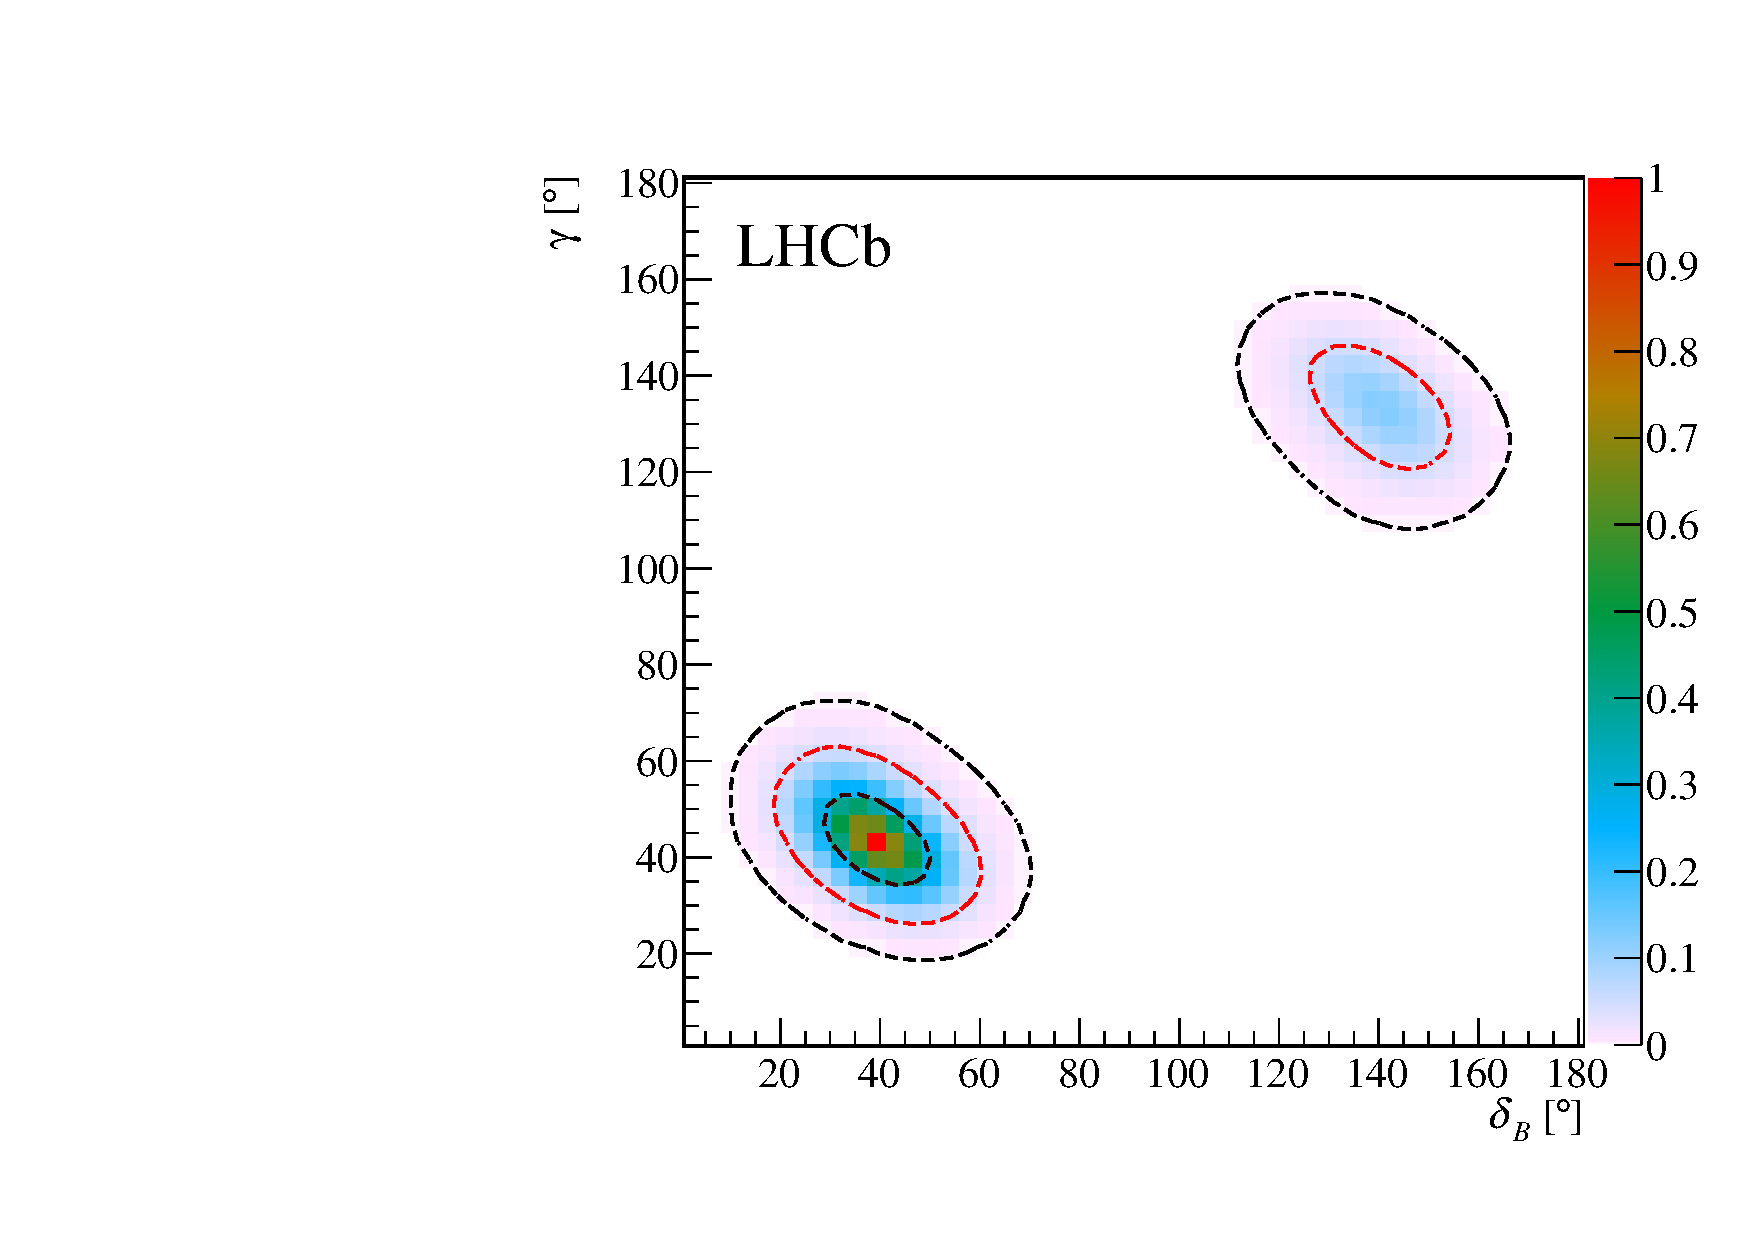
\includegraphics[width=0.5\linewidth]{figures/interpretation/deltaBu_dkstar_gamma_2Dscan_nomixing_endofrun3.pdf}}
\caption{2D contour plots projected to the end of Run 3 assuming the central values remain the same.}
\label{gammadiniplotsrun3}
\end{figure}


\clearpage
